\documentclass[a4paper,11pt]{article}
\usepackage{amsmath,amsthm,amsfonts,amssymb,amscd,amstext,vmargin,graphics,graphicx,tabularx,multicol} 
\usepackage[francais]{babel}
\usepackage[utf8]{inputenc}  
\usepackage[T1]{fontenc} 
\usepackage{pstricks-add,tikz,tkz-tab,variations}
\usepackage[autolanguage,np]{numprint} 
\usepackage{calc}
\usepackage{fp}

\setmarginsrb{1.5cm}{0.5cm}{1cm}{0.5cm}{0cm}{0cm}{0cm}{0cm} %Gauche, haut, droite, haut
\newcounter{numexo}
\newcommand{\exo}[1]{\stepcounter{numexo}\noindent{\bf Exercice~\thenumexo} : }
\reversemarginpar

\newcommand{\bmul}[1]{\begin{multicols}{#1}}
\newcommand{\emul}{\end{multicols}}

\newcounter{enumtabi}
\newcounter{enumtaba}
\newcommand{\q}{\stepcounter{enumtabi} \theenumtabi.  }
\newcommand{\qa}{\stepcounter{enumtaba} (\alph{enumtaba}) }
\newcommand{\initq}{\setcounter{enumtabi}{0}}
\newcommand{\initqa}{\setcounter{enumtaba}{0}}

\newcommand{\be}{\begin{enumerate}}
\newcommand{\ee}{\end{enumerate}}
\newcommand{\bi}{\begin{itemize}}
\newcommand{\ei}{\end{itemize}}
\newcommand{\bp}{\begin{pspicture*}}
\newcommand{\ep}{\end{pspicture*}}
\newcommand{\bt}{\begin{tabular}}
\newcommand{\et}{\end{tabular}}
\renewcommand{\tabularxcolumn}[1]{>{\centering}m{#1}} %(colonne m{} centrée, au lieu de p par défault) 
\newcommand{\tnl}{\tabularnewline}

\newcommand{\trait}{\noindent \rule{\linewidth}{0.2mm}}
\newcommand{\hs}[1]{\hspace{#1}}
\newcommand{\vs}[1]{\vspace{#1}}

\newcommand{\N}{\mathbb{N}}
\newcommand{\Z}{\mathbb{Z}}
\newcommand{\R}{\mathbb{R}}
\newcommand{\C}{\mathbb{C}}
\newcommand{\Dcal}{\mathcal{D}}
\newcommand{\Ccal}{\mathcal{C}}
\newcommand{\mc}{\mathcal}

\newcommand{\vect}[1]{\overrightarrow{#1}}
\newcommand{\ds}{\displaystyle}
\newcommand{\eq}{\quad \Leftrightarrow \quad}
\newcommand{\vecti}{\vec{\imath}}
\newcommand{\vectj}{\vec{\jmath}}
\newcommand{\Oij}{(O;\vec{\imath}, \vec{\jmath})}
\newcommand{\OIJ}{(O;I,J)}

\newcommand{\droite}[2]{
  \psline{->}(0,0)(#2,0)
\FPdiv{\division}{1}{#1}%Variable pour la division de la longueur Unit\'e.
\FPmul{\produit}{#1}{#2}%Variable pour les graduations sur toute la longueur de l'axe.
\FPclip{\produit}{\produit}%Supression des z\'eros inutiles.
  \multido{\r=0+\division}{\produit}%Boucle PsTricks
  {
  \psline(\r,-0.075)(\r,0.075)
  }
}

%\droite gradu\'ee avec nombres{Nb de divisions de la longueur unit\'e}{longueur axe}
\newcommand{\droitenombres}[2]{
  \psline{->}(0,0)(#2,0)
\FPdiv{\division}{1}{#1}
\FPmul{\produit}{#1}{#2}
\FPclip{\produit}{\produit}
  \multido{\r=0+\division}{\produit}
  {
  \psline(\r,-0.075)(\r,0.075)
  }
\multido{\i=0+1}{#2}{
\psline[linewidth=0.03](\i,-0.15)(\i,0.15)
\rput(\i,0.35){\i}}
}

%\droite gradu\'ee avec nombres{Nb de divisions de la longueur unit\'e}{longueur axe}{nb d\'epart}
\newcommand{\droitenombresorigine}[3]{
  \psline{->}(0,0)(#2,0)
\FPdiv{\division}{1}{#1}
\FPmul{\produit}{#1}{#2}
\FPclip{\produitentier}{\produit}
  \multido{\r=0+\division}{\produitentier}
  {
  \psline(\r,-0.075)(\r,0.075)
  }

\FPset{\nbchoisi}{#3}
\multido{\i=0+1}{#2}{
\psline[linewidth=0.03](\i,-0.15)(\i,0.15)
\rput(\i,0.35){\nbchoisi}
\FPadd{\nbchoisi}{1}{\nbchoisi}
\FPclip{\nbchoisi}{\nbchoisi}
}
}


%\droite gradu\'ee avec nombres{Nb de divisions de la longueur unit\'e}{longueur axe}{nb d\'epart}{pas}
\newcommand{\droitenombresoriginepas}[4]{
  \psline{->}(0,0)(#2,0)
\FPdiv{\division}{1}{#1}
\FPmul{\produit}{#1}{#2}
\FPclip{\produitentier}{\produit}
  \multido{\r=0+\division}{\produitentier}
  {
  \psline(\r,-0.075)(\r,0.075)
  }
\FPset{\nbchoisi}{#3}
\multido{\i=0+1}{#2}{
\psline[linewidth=0.03](\i,-0.15)(\i,0.15)
\rput(\i,0.35){\nbchoisi}
\FPadd{\nbchoisi}{#4}{\nbchoisi}
\FPclip{\nbchoisi}{\nbchoisi}
}
}
\newcommand{\reponse}[1][1]{%
\multido{}{#1}{\makebox[\linewidth]{\rule[0pt]{0pt}{20pt}\dotfill}
}}

\newcommand{\titre}[5] 
% #1: titre #2: haut gauche #3: bas gauche #4: haut droite #5: bas droite
{
\noindent #2 \hfill #4 \\
#3 \hfill #5

\vspace{-1.6cm}

\begin{center}\rule{6cm}{0.5mm}\end{center}
\vspace{0.2cm}
\begin{center}{\large{\textbf{#1}}}\end{center}
\begin{center}\rule{6cm}{0.5mm}\end{center}
}



\begin{document}
\pagestyle{empty}
\titre{Séance d'AP . . . : Repérage sur une demi-droite graduée}{}{}{6ème}{}

\vspace*{0.2cm}

\setlength{\fboxrule}{2pt}
\begin{flushleft}
\framebox{\begin{minipage}{\linewidth}

\vspace*{0.5cm}

\underline{\textbf{COURS}}\\

{\large \textbf{{\textcolor{green}{\underline{Définition 1 :}}}}}
\textbf{Une demi-droite graduée} est une demi-droite sur laquelle on a choisi une unité de longueur que l'on reporte régulièrement à partir de \textbf{l'origine}.

\begin{center}
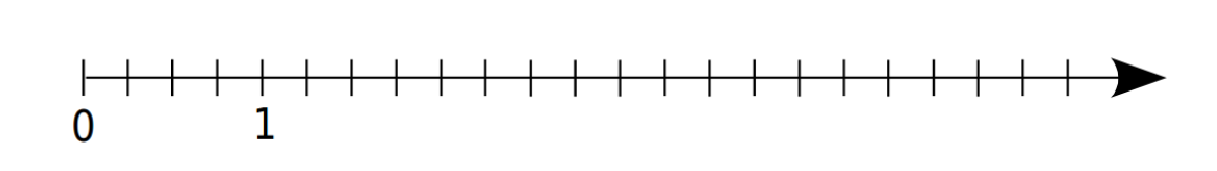
\includegraphics[scale=0.7]{abscisse10.eps} 
\end{center}

\vspace*{1cm}


{\large \textbf{{\textcolor{green}{\underline{Définition 2 :}}}}} \textbf{L'abscisse d'un point} est le nombre qui repère ce point sur une demi-droite graduée.\\


Par exemple, sur la demi-droite au-dessus :
l'abscisse du point H est . . . et l'abscisse du point M est . . .\\



\vspace*{0.5cm}
\end{minipage}}
\end{flushleft}

\vspace*{1cm}





\bmul{2}

\exo\\
 Écrire les abscisses des points de chaque demi-droite graduée.

\begin{flushleft}
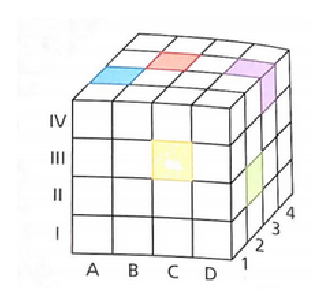
\includegraphics[scale=0.75]{reperage1.eps} 
\end{flushleft}

\columnbreak

\exo \\
Placer les points, le plus précisément possible, sur les demi-droites graduées.	

\begin{flushleft}
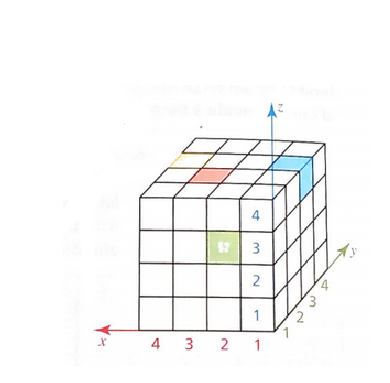
\includegraphics[scale=0.87]{reperage2.eps} 
\end{flushleft}

\emul

\vspace*{0.5cm}

\exo \\ Placer les points d'abscisses suivants :
\begin{flushleft}
 A( 2 unités et 1 dixièmes )		 \hspace*{0.35cm}  B(11 dixièmes) \hspace*{0.35cm} C($\dfrac{17}{10}$) \hspace*{0.35cm} D(40 centièmes ) \hspace*{0.35cm}  E($2 + \dfrac{2}{10}$) \hspace*{0.35cm} F(145 centièmes)
\end{flushleft}


\begin{center}
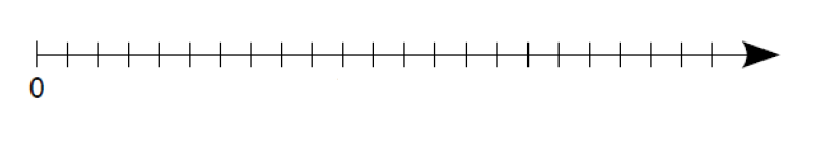
\includegraphics[scale=0.9]{reperage3.eps} 

\end{center}




\end{document}
